\chapter{Preliminares}\label{chapter:state-of-the-art}
\section{Tipos de contraseñas gráficas}
La amplia gama de contraseñas gráficas disponibles se puede organizar en una clasificación que facilita su estudio y comparación. A continuación, se presenta el análisis de cuatro categorías que abarcan la mayoría de los enfoques existentes: contraseñas basadas en el reconocimiento, las cuales dependen de la identificación de elementos visuales; contraseñas basadas en el dibujo, donde el usuario crea un patrón personalizado; contraseñas basadas en \textit{Clicks}, que utilizan la selección secuencial de puntos en una pantalla; y, por último, los esquemas híbridos, que combinan elementos de las categorías anteriores. Cada una de estas categorías representa un enfoque distinto en cuanto a la interacción del usuario y presenta diferentes ventajas y desventajas en términos de seguridad y usabilidad.  
\subsection{Contraseñas basadas en reconocimiento}
Los sistemas basados en el reconocimiento son aquellos donde el usuario debe reconocer su contraseña de entre un conjunto de otras contraseñas o elementos distractorios, de tal forma que solo el usuario auténtico sea capaz de acceder al recurso protegido.

 
El sistema \textit{Deja Vu}, desarrollado por \cite{dhamija2000deja}, ilustra un enfoque de contraseña gráfica basado en reconocimiento. En este esquema, el usuario configura su contraseña seleccionando un conjunto de imágenes que conforman un portafolio, como muestra el Anexo No. \ref{figure:deja-vu}. El proceso de autenticación requiere que el usuario identifique correctamente las imágenes de su portafolio, las cuales se presentan mezcladas con imágenes señuelo. Para garantizar la memorabilidad de la contraseña se pide hacer un pequeño entrenamiento por parte del usuario, en el que deberá identificar las imágenes del portafolio de un conjunto con imágenes señuelo, esto disminuye la experiencia de usuario en la fase de registro. Este sistema aprovecha la habilidad humana para recordar imágenes previamente vistas, lo que, según \cite{dhamija2000deja}, las hace más resistentes a ataques de ingeniería social al dificultar la elección de contraseñas débiles y su intercambio.


\textit{Pass Faces} \cite{Tuscano2015GraphicalPA}, \cite{inproceedings} es otro ejemplo de sistemas basados en el reconocimiento, esta vez basado en la capacidad de reconocimiento facial. En este sistema el usuario debe seleccionar un conjunto de caras, al igual que en el anterior, en el momento de autenticación el usuario debe seleccionar 4 caras de una cuadrícula de 3x3 caras como muestra el Anexo No. \ref{passfaces}. En \cite{Tuscano2015GraphicalPA} se ha demostrado que este sistema es predecible, pues la selección de las caras está sujeta a características étnicas, raciales o tendencias a seleccionar caras más atractivas.





\subsection{Contraseñas basadas en dibujo}
En contraste, las contraseñas basadas en dibujo son aquellas donde se le pide al usuario dibujar a mano su contraseña, con el objetivo de reconocer los trazos o secuencias que cree el mismo. Están inspirados en las firmas que se utilizan para garantizar la veracidad de las personas en documentos oficiales o elementos similares. 

Un ejemplo muy conocido de este tipo de contraseña gráfica,son los patrones de desbloqueo de \textit{Android}, permiten al usuario crear un patrón enlazando puntos en una cuadrícula como se ve en la figura \ref{android-pattern}. Estos patrones de desbloqueo presentan vulnerabilidades como los ataques de \emph{Smudge} \cite{aviv2010smudge}, ataques que se basan en las marcas de grasa o suciedad que se encuentran en la pantalla despu\'es de colocado el patr\'on, ver figura \ref{smudge-screen} y una reducción del espacio de contraseñas al no permitir la repetición de puntos. Otra vulnerabilidad de este sistema  es ante el ataque \emph{Shoulder Surfing}, este consiste en que un atacante observa, graba o registra los eventos de la pantalla del usuario mientras este dispone su contraseña durante fase de registro o autenticación.






\textit{Free Form Draw} \cite{lin2009free} ofrece mayor libertad al permitir dibujar cualquier figura y registrarla como contraseña, pues se basa en la idea de que los trazos son únicos para cada individuo. Dicho dibujo debe ser reproducido durante la fase de autenticación. En \cite{lin2009free} siguen la premisa de que un usuario al escribir o dibujar realiza los trazos de forma inconsciente y automatizada, una persona deja no solo su estado mental, sino un estado de la consciencia por lo que se tiene el dibujo resultante como: ``un diagrama del inconsciente``.

Dibujar exactamente lo mismo con precisión quirúrgica en el momento de reproducir cada trazo es prácticamente imposible, es necesario tener una forma de verificar todos los posibles futuros dibujos que el usuario utilizará en la fase de autenticación. 
Para esto se le pide al usuario ingresar durante la fase de registro su contraseña o firma digital varias veces, ver figuras \ref{free-draw-train-mouse} y \ref{free-draw-train-stylus}, esto se procesa y se utiliza un modelo de Regresión Polinomial \cite{heiberger2009polynomial} para poder predecir y verificar la contraseña del usuario en caso de que sus trazos tengan muchas fluctuaciones, ver figura \ref{free-form-draw-polinomial}.  Si la cantidad de fluctuaciones es mayor, se utiliza un modelo de regresión B-spline \cite{imoto2000b}, este fusiona la suavidad polinomial y la precisión de la influencia local de la aproximación o interpolación lineal, ver figura \ref{free-form-draw-spline}.





\subsection{Contraseñas basadas en \textit{Clicks}}
Las contraseñas basadas en \textit{Clicks} se basan en la selección de elementos en un orden específico solo conocido por el usuario auténtico. 
Ejemplos son las contraseñas basadas en historias o narrativas \cite{olade2023story}, \cite{hoover2015narrative}, donde se seleccionan puntos en imágenes semánticamente relacionadas para crear una historia. En el caso de  \textit{Semantic Lock} \cite{olade2023story} definen una contraseña como una secuencia de $k$ imágenes seleccionadas de un conjunto de $n > k$ imágenes, dichas $k$ imágenes deben estar dispuestas por el usuario de forma que su unión y orden represente una historia, ver figura \ref{semantic-passw}.

\textit{Passpoints} \cite{wiedenbeck2005passpoints} fue diseñado en el 2005 por Susan Wiedenbeck, inspirado en el modelo propuesto por Blonder \cite{blonder1996graphical}, basa su funcionamiento en que un usuario seleccione un conjunto ordenado de 5 puntos en una imagen como su contraseña en la fase de registro.

\textit{Cued Click Points} \cite{chiasson2007graphical} propone una mejora al modelo anterior en cuanto a usabilidad, seleccionando un punto por cada imagen de un conjunto de imágenes en lugar de varios puntos de una misma imagen. Sin embargo, esto aumentaría la carga computacional de una implementación de dicho sistema.

De \textit{Passpoinst} se han derivado variantes como \textit{PassPositions} y \textit{PassPositions} 2 \cite{8320723}, que agregan información posicional para aumentar la seguridad y fortaleza ante ataques de diccionario. Logran esto haciendo que el cálculo del \textit{hash} de un punto se haga tomando como referencia la posición del anterior como se puede ver en el Anexo No. \ref{passpositions-example}.




\textit{Pass Maps} \cite{10.1145/2414456.2414513}, emplea un mapa mundial para aumentar el espacio de contraseñas, ver figura \ref{passmap}, por tanto, aumenta también su resistencia ante ataques de diccionario o fuerza bruta \cite{5738831}.



Otro esquema basado en \textit{clicks} es \textit{PassGo} \cite{tao2008pass}, inspirado en el juego ``Go``. En este los usuarios deben selecccionar intersecciones en una cuadrícula. Cada intersección tiene un área sensible alrededor para compensar pequeñas inexactitudes en la entrada del usuario. Se muestran indicadores de puntos y líneas para las intersecciones seleccionadas y las líneas dibujadas entre ellas, ver figura \ref{go-passwords}. Luego la contraseña se codifica como una secuencia de pares de coordenadas bidimensionales.



\subsection{Esquemas Híbridos}
Los esquemas híbridos, como \textit{Gra-Pin} \cite{kausar2022gra} o \textit{PassMatrix} \cite{8250568}, combinan diferentes enfoques de contraseñas gráficas (incluso con alfanuméricas), como la combinación de un PIN con la selección de imágenes o la selección de secuencias de imágenes como un PIN. 

En el caso de \textit{Gra-Pin} \cite{kausar2022gra} se pide al usuario seleccionar un número secreto de 2 dígitos, luego se le pide seleccionar una imagen secreta de entre otras 9 opciones, se pide seleccionar una operación aritmética y una posición secreta para  un Pin. 

Esta combinación de elementos compone su contraseña. En la fase de autenticación, se pide al usuario contar cuántas veces aparece su imagen secreta en una cuadrícula de 5x5 imágenes. Realiza la operación aritmética seleccionada en la fase anterior entre el número de veces que aparecía su imagen secreta y el número secreto de dos cifras seleccionado durante el registro, por último se pone el resultado de esta operación en la posición seleccionada en el registro en el Pin, poniendo el resto de dígitos aleatorios como se puede ver en las figuras \ref{gra-pin} y \ref{gra-pin-screens}. 

Este método está diseñado para mantener la resistencia que las contraseñas gráficas ofrecen y presentan adem\'as mayor resistencia ante ataques de tipo \textit{Shoulder Surfing} 
 \cite{lashkari2009shoulder}






\section{\textit{Passpoints}}

Como se mencionó anteriormente, el sistema \textit{Passpoinst} \cite{wiedenbeck2005passpoints} se basa en la memorización de una secuencia de cinco puntos seleccionados en una imagen durante la fase de registro, como se muestra en la figura \ref{passpoints-example}

\begin{figure}[H]
	\centering
		\begin{minipage}[b]{0.7\linewidth}  % Tercer cuadrado, 48% del ancho de línea
		\centering
		\adjustbox{valign=b}{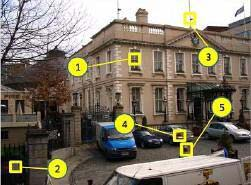
\includegraphics[width=0.8\linewidth]{passpoints.jpg}} % valign=t para alinear la imagen en la parte superior
		\caption{Ejemplo de Passpoints, Fuente: \cite{wiedenbeck2005passpoints}}
		\label{passpoints-example}
	\end{minipage}%
	
\end{figure}
. En la fase de autenticación el usuario tendrá  que  seleccionar dichos puntos en el mismo orden que en la fase de registro. En  este  sistema  cualquier  imagen  puede  ser  utilizada  (pinturas,  fotos  naturales,  fotos  familiares,  etc),  y  puede  ser seleccionada  por  el  usuario  o proveídas por  el  sistema.  La  imagen  debe  tener  cientos  de  puntos  probables  de  ser seleccionados y deben estar diseminados de forma homogénea para mayor seguridad.
 
Por motivos de seguridad, el sistema  no  almacena  de  forma explícita la contraseña,  sino  un hash  de la  misma,  esto  trae  consigo  el  problema de identificar el usuario legítimo, ya que es muy poco probable que se digiten exactamente los mismos puntos durante las fases de registro y autenticación, haciendo que los hashes sean diferentes. 
Para solventar este problema es necesario agregar un margen de error para la selección de los puntos, concidos como región de tolerancia. Para lograr esto se utiliza una discretización de la imagen, lo que reduce el espacio de contraseñas y aporta información relevante para  llevar  a  cabo  ataques  de  diccionario \cite{zhu2013security}. Además  permite  la  aparición  de  falsos  positivos  y negativos  en  la autenticación  debido  a  la  forma  de  las  regiones  calculadas  utilizando  la  discretización. 

 Una  discusión  acerca  de  la importancia del mecanismo de discretización en los esquemas de contraseñas gráficas y de los diferentes métodos de discretización conocidos hasta el momento puede verse en \cite{birget2006graphical}, \cite{chiasson2008centered}, \cite{bicakci2008optimal}, \cite{kirovski2007click}. 

Otros aspectos negativos a destacar en este sistema son: 

\begin{itemize}
	\item Algunas regiones en la imagen son más propensas a ser seleccionadas por el usuario para formar su contraseña \cite{mypasswordhere}.
	
	\item Dado que este sistema basa su funcionamiento en la selección de 5 puntos en la imagen, la fase de registro y de autenticación pueden extenderse lo que conlleva a que sean vulnerables ante ataques de tipo \textit{Shoulder-Surfing} \cite{rodriguez2019algoritmo}.
	
	\item Si el conjunto de puntos seleccionados por el usuario no sigue un patrón aleatorio es considerada débil y es susceptible a ataques de diccionarios \cite{rodriguez2019algoritmo}.
\end{itemize}

En varios artículos publicados recientemente \cite{sym13050777}, \cite{lissetMaster}, \cite{s22051987}, \cite{herrera2023comparacion}, \cite{herrera2023nuevo}, \cite{herrera2023nuevoregulares}, \cite{herrera2024new} se proponen test para evitar el registro de contraseñas gráficas no aleatorias. Estos resultados unidos a la propuesta en \cite{legon2019nuevo} de un modelo probabilístico capaz de medir el nivel de autenticidad de un usuario, conllevan a un aumento significativo en la seguridad de este sistema y por consiguiente lo convierten en una de las alternativas más prometedoras ante las contraseñas alfanuméricas.



\subsection{¿Por qué usar \textit{Passpoints}?}

La notoria falta de seguridad de las contraseñas alfanuméricas, debido a la contradicción que presentan las mismas \cite{zimmermann2020password}, es una señal de que se requieren opciones más seguras y sencillas de usar. En este escenario, el sistema \textit{Passpoints} se erige como una buena alternativa a las tradicionales contraseñas alfanuméricas. La seguridad de este método de autenticación gráfica reside en su espacio de contraseñas \( Q^L \), donde \( Q \) es el tamaño del alfabeto y \( L \) la longitud de la contraseña \cite{legon2019nuevo}. Mientras que en el caso de las contraseñas alfanuméricas este espacio consiste en la cantidad de cadenas que se pueden formar con un alfabeto específico, en \textit{Passpoints} es la cantidad de combinaciones de puntos (píxeles) de la imagen que se utilice.

En la actualidad, los tamaños de imágenes que se manejan rondan los cientos de miles de píxeles, lo que incrementa aún más el espacio de contraseñas de \textit{Passpoints}. Esto tiene un impacto positivo en su nivel de seguridad y resistencia a ataques de fuerza bruta. Al ser un método novedoso y poco conocido, no existen grandes bases de datos de contraseñas \textit{Passpoints}, a diferencia de la enorme cantidad de información y recopilaciones de contraseñas alfanuméricas disponibles en Internet. Esta falta de información le otorga una mayor resistencia a \textit{Passpoints} ante ataques de diccionario \cite{weakpassw}.

Además, al explotar la capacidad humana de reconocer patrones en imágenes, \textit{Passpoints} facilita el recuerdo de las contraseñas para cualquier tipo de persona, desde niños y adolescentes hasta personas de la tercera edad. Esto contrasta con las contraseñas alfanuméricas, donde, para garantizar la seguridad, se hace necesario que los usuarios memoricen largas cadenas con altos niveles de aleatoriedad. En \cite{rodriguez2018seguridad} se ratifica la posición de \textit{Passpoints} como el método de autenticación gráfica más conveniente, a través de una comparación y evaluación crítica de los diferentes métodos existentes.

\subsection{Región de Tolerancia}
La región de tolerancia \cite{legon2019nuevo, borrego2018debilidades} de un punto \(p\) se define como el conjunto de puntos de la imagen que son aceptados como válidos durante la autenticación para el punto original \(p_0\), y se denota como \(R_T\). Sea \(I\) el conjunto de píxeles de la imagen, y \(f\) una función tal que para todo punto de la imagen devuelve 1 si es aceptado y 0 en caso contrario. Entonces, \(R_T\) quedaría definido como:

\begin{equation}
	R_T = \{p, p \in I \cap f(p) = 1\} \label{eq:region_tolerancia}
\end{equation}

Puede interpretarse la región de tolerancia como el error permitido al usuario en el momento de seleccionar su contraseña.

\subsubsection{Punto \texorpdfstring{$r$}{r}-seguro}
Un punto se considera $r-seguro$ \cite{legon2019nuevo,  borrego2018debilidades} para un radio \(r\) si y solo si todo punto que está a una distancia \(r\) de él se incluye en la región de tolerancia. Sea \(I\) el conjunto de píxeles de una imagen, \(p_0\) un punto de la imagen y \(R_T\) la región de tolerancia. Se dice que \(p_0\) es $r-seguro$ si y solo si:
\begin{equation}
	\forall p \in I: d(p_0, p) < r \Rightarrow p \in R_T \label{eq:r_seguro}
\end{equation}
		
\begin{figure}[h]
			\centering
			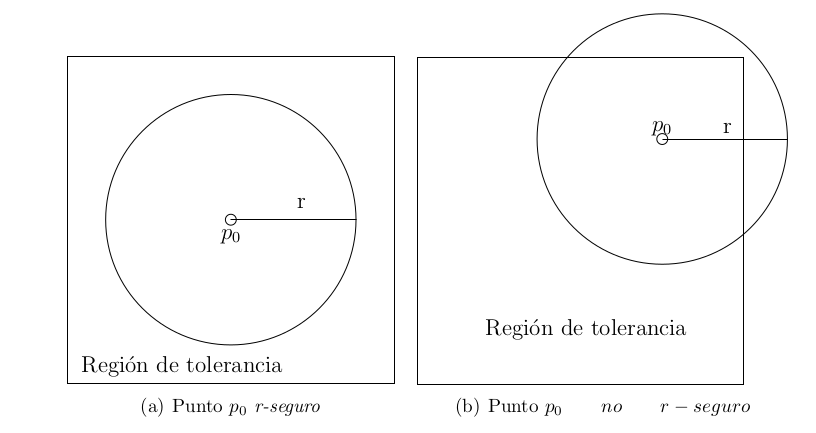
\includegraphics[width=0.5\textwidth]{punto-r-seguro.png}			
			\caption{Ejemplo de punto $r-seguro$ y punto no $r-seguro$, Fuente: \cite{legon2019nuevo} }
		\end{figure}
		
	
\subsection{Problema del Vértice}
Este problema surge durante la fase de registro \cite{legon2019nuevo, birget2006graphical, borrego2018debilidades}, cuando el usuario puede seleccionar un punto que no es $r-seguro$. Hay dos casos posibles: seleccionar un punto localizado exactamente en los vértices o aristas de la región de la partición, o seleccionar un punto que está situado a una distancia \(d < r\) de los mismos. El primer caso plantea un problema de decisión para determinar la región de tolerancia del punto. Es necesario discretizar las imágenes de tal manera que cada punto pertenezca a una región de tolerancia.
	
\subsection{Problema del Hash}
Por temas de seguridad, las contraseñas no pueden almacenarse en texto claro. Es necesaria una forma segura de representarlas tal que para cada contraseña exista un identificador único y que estas no sean recuperables desde dicho identificador. Las funciones \textit{hash} \cite{legon2019nuevo, borrego2018debilidades} encajan perfectamente con esta definición, por lo que son un buen recurso a utilizar para almacenar las contraseñas. Sin embargo, usando un \textit{hash} surge la problemática de que cada punto de la región de tolerancia tendrá un \textit{hash} diferente, impidiendo así que guardar el \textit{hash} de los puntos seleccionados sea una buena opción. Utilizando como parámetro de la función \textit{hash} no solo un punto, sino toda su región de tolerancia, no solo se garantiza que se puedan guardar los \textit{hashes} de las contraseñas, sino que también aumenta la cardinalidad del espacio de entrada de la función \textit{hash}, lo que dificulta los ataques de fuerza bruta.
	
\subsection{M\'etodos de Discretizaci\'on}	
Es sencillo percatarse de la baja probabilidad de que un usuario seleccione siempre exactamente el mismo pixel en las fases de registro y autenticación, situación que se agrava aún más en escenarios como el de los teléfonos móviles, cajeros y otras situaciones donde el usuario no posee un puntero digital. Es por  esto que se hace necesario dar un margen de error a cada punto de la contraseña Passpoints, a la región definida por el punto y su margen de error se le conoce como región de tolerancia. Una forma eficiente y segura de introducir esta región de tolerancia en un sistema de autenticación gráfica \textit{Passpoints} es utilizando una discretización.
\subsubsection{Discretización Robusta}

Para evitar el problema del vértice \cite{birget2006graphical}, se utiliza un conjunto de tres particiones diferentes de la imagen. Esto garantiza que cada punto es $r-seguro$ en al menos una de dichas particiones. Esto se logra asegurando una separación de al menos r píxeles entre el punto y el borde de alguna de las tres particiones \cite{zhu2013security, chiasson2008centered}. Se toman cuadrículas de dimensiones \(6r \times 6r\) y cada partición debe estar separada una distancia \(2r\) del resto. Durante la fase de autenticación, debido a la construcción de las particiones, cualquier punto a una distancia \(d \leq r\) del punto original pertenecerá al mismo cuadrante, lo que garantiza la autenticación del usuario ya que la salida de la función \textit{hash} será la misma. Por otro lado, cualquier punto a una distancia mayor a \(5\sqrt{2}r\) pertenecerá a otro cuadrante, lo que garantiza la no autenticación del usuario ilegítimo.

		\begin{figure}[H]
			\centering
			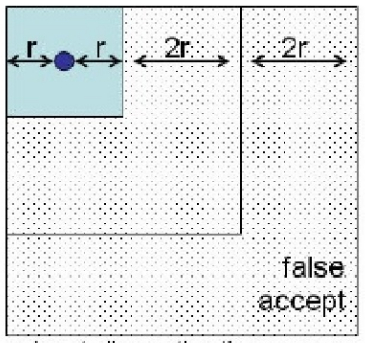
\includegraphics[width=0.25\textwidth]{image4.jpg}
			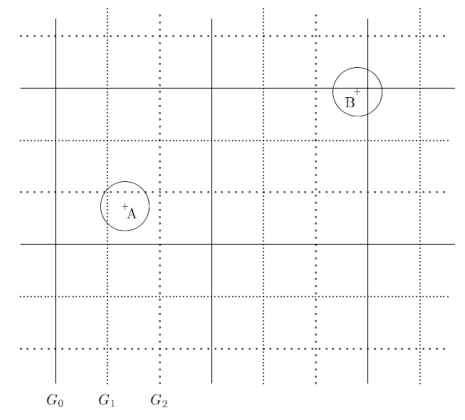
\includegraphics[width=0.3\textwidth]{image2.png}
			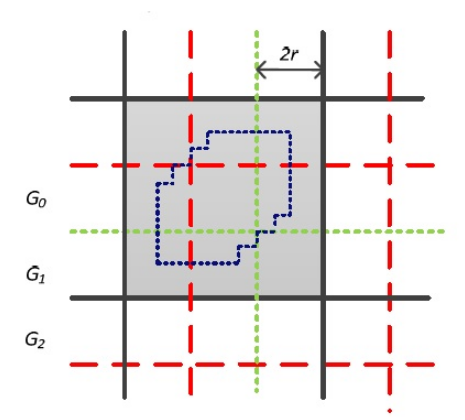
\includegraphics[width=0.3\textwidth]{image3.png}
			\caption{Regiones de la discretizaci\'on robusta, Fuentes: \cite{zhu2013security} y \cite{chiasson2008centered}.}
		\end{figure}
	
\subsubsection{Discretización Centrada}
	
La Discretización Centrada \cite{chiasson2008centered} ofrece mejoras en usabilidad y seguridad en comparación con la discretización robusta. Esta técnica garantiza que la región de tolerancia esté centrada en el punto seleccionado para la contraseña, resolviendo así el problema del vértice. Al determinar una región de dimensiones \(2r \times 2r\) centrada en el punto. Este método funciona encontrando, en cada dimensión de la imagen (\textit{x}, \textit{y}), un segmento de longitud \(2r\) en el cual el centro sea el punto originalmente seleccionado en el registro. Sea \textit{x} un punto en la semirrecta numérica que comprende los valores entre 0 y \textit{m}, donde \textit{m} es el ancho o largo de la imagen, dependiendo de la dimensión que se quiera calcular. A partir de ese segmento, se divide el resto del intervalo $[0, m]$ en subintervalos de igual longitud.

En la mayoría de los casos, habrá sobrantes de tamaño \(d\), donde \(d\) pertenece al intervalo $[0, 2r]$, por lo que si se almacena el valor de \(d\) es posible reconstruir la partición realizada comenzando en \(d\), donde uno de estos subintervalos estará centrado en \textit{x}. Una vez establecido el radio \textit{r} y el punto de la contraseña \textit{x}, se puede calcular la región de tolerancia. Se calcula el sobrante \textit{d} que se utilizará luego en la fase de autenticación:
\begin{equation}
	d \equiv (x - r) \pmod{2r} \label{eq:sobrante}
\end{equation}

Determinar el intervalo exacto \textit{i} donde se encuentra \textit{x}:
\begin{equation}
	i = \left\lfloor \frac{x - r}{2r} \right\rfloor \label{eq:intervalo_registro}
\end{equation}

Una vez seleccionado el punto \textit{x'} durante la fase de autenticación, se halla el intervalo \textit{i'} donde este se encuentra:
\begin{equation}
	i' = \left\lfloor \frac{x' - r}{2r} \right\rfloor \label{eq:intervalo_autenticacion}
\end{equation}
Nótese que \textit{i} no está centrado en \textit{x'}, pero \(|x - x'| < r \rightarrow i = i'\). Por tanto, se utiliza \textit{i} como componente de la contraseña.

	\begin{figure}[H]
		\centering
		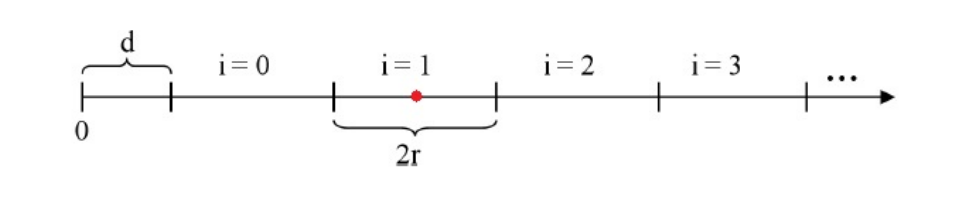
\includegraphics[width=0.9\textwidth]{image5.png}	
		\caption{Ejemplo de recta num\'erica discretizada. centralmente. Fuente: \cite{bicakci2008optimal}}	
	\end{figure}

Este método de autenticación supone una mejora sustancial en cuanto a su complejidad de implementación, ya que elimina la necesidad de crear varias particiones en la imagen. Sin embargo, este método introduce un nuevo problema: la necesidad de almacenar el valor \textit{d} en texto claro para poder efectuar la autenticación correctamente. Una posible solución a este problema sería encriptar este valor de forma reversible y almacenarlo junto al \textit{hash} de la contraseña concatenándolo al mismo. Esto permitiría al sistema, durante la fase de autenticación, recuperar estos datos y determinar si los puntos seleccionados son válidos o no.


\subsubsection{Discretización Óptima}
	
Este método mantiene la filosofía de particionar la imagen generando una región centrada en el punto original de la contraseña, pero utiliza propiedades de la aritmética modular para construirla \cite{bicakci2008optimal}. Sean \textit{r} el radio de tolerancia y \textit{X} el punto seleccionado por el usuario, se calcula:
\begin{equation}
	\begin{aligned}
		\textit{X} \mod{2r} \geq r &\rightarrow \phi \equiv X \mod{r} \\
		\textit{X} \mod{2r} < r &\rightarrow \phi \equiv (X \mod{2r}) - r
	\end{aligned}
	\label{eq:phi}
\end{equation}
De forma análoga se calcula:
\begin{equation}
	\begin{aligned}
		\textit{Y} \mod{2r} \geq r &\rightarrow \varphi \equiv Y \mod{r} \\
		\textit{Y} \mod{2r} < r &\rightarrow \varphi \equiv (Y \mod{2r}) - r
	\end{aligned}
	\label{eq:varphi}
\end{equation}
Estos valores (\(\phi\)) y (\(\varphi\)) se almacenan en claro en el sistema junto a los \textit{hashes}:
\begin{equation}
	S_X = \frac{X - \phi}{2r}, \quad S_Y = \frac{Y - \varphi}{2r} \label{eq:hashes}
\end{equation}

Durante la fase de autenticación, el usuario selecciona el píxel (\textit{X'}, \textit{Y'}), utilizando los valores de (\(\phi\)) y (\(\varphi\)) almacenados para ese usuario se calculan los \textit{hashes} \(S_{X'}\) y \(S_{Y'}\) cumpliéndose que se garantiza la autenticación.
\begin{equation}
	\|(X, Y) - (X', Y')\| < r \rightarrow S_{X'} = S_X \land S_{Y'} = S_Y \label{eq:autenticacion}
\end{equation}
Este método es más eficiente que los descritos anteriormente, ya que su implementación a nivel computacional tiene una menor complejidad. Al tomar como base la aritmética modular se reduce la complejidad de los cálculos necesarios. No soluciona el problema del anterior método debido a que mantiene la necesidad de guardar texto claro junto con  las  contraseñas,  en  este  caso  son  los  valores   ($\phi$)  y  ($\varphi$).  Aunque  esto tiene  una  solución  rápida  que comparte con la discretización centrada

\subsubsection{Discretización mediante polígonos de Voronoi}
Otras propuestas de discretización encontradas en la bibliografía es la hecha por Kirovski et al. \cite{kirovski2007click}, donde proponen utilizar diagramas de Voronoi. Partiendo de los puntos más probables de ser seleccionados en la imagen (conocidos como \textit{Hotspots} en la literatura), propone aplicar una discretización de Voronoi ponderada usando una heurística para maximizar la entropía \(H(P_w)\), tratando de obtener polígonos equiprobables. Su ventaja principal es que todos los polígonos de la partición obtenida poseen aproximadamente la misma probabilidad a priori de que el usuario escoja un punto de ese polígono. Esta propiedad parece ofrecer mejor resistencia a los ataques de diccionario basados en \textit{Hotspots}. Sin embargo, en \cite{zhu2013securityl} se afirma que la propuesta de \cite{kirovski2007click} sigue dejando información en claro, útil para ataques de diccionario.

\subsubsection{Problemas de los métodos de discretización}
	
El uso de los métodos de discretización conlleva a ciertas limitaciones durante la autenticación. Una de estas es la falta de diferenciación entre los puntos que se encuentran dentro de la región de tolerancia. Todos los puntos reciben el mismo tratamiento, lo cual contradice el comportamiento esperado por parte del usuario legítimo, que debería seleccionar con mayor frecuencia los puntos más cercanos al punto original. Además, al representar la región de tolerancia como un polígono en lugar de un círculo, existe la posibilidad de obtener falsos positivos, es decir, puntos que se encuentran a una distancia mayor que el radio de tolerancia establecido pero que aún se consideran válidos como parte de la contraseña \cite{blonder1996graphical, borrego2018debilidades}. Otro problema se presenta cuando existen puntos situados a la misma distancia del punto seleccionado como parte de la contraseña, siendo ambos válidos para el usuario legítimo. Sin embargo, uno de ellos puede quedar dentro de la región de tolerancia determinada por la discretización y el otro no, lo que genera falsos negativos. Además, al segmentar la imagen en cuadrículas, no se toman todos los puntos que deberían determinar la región de radio \textit{r} alrededor del punto seleccionado como contraseña. Esto puede afectar la experiencia de usuario al utilizar el sistema \cite{bicakci2008optimal, borrego2018debilidades}.

En general, las limitaciones de los métodos de discretización radican en el hecho de que definen la región de tolerancia como un polígono, mientras que la distancia se plantea en términos de un círculo. Además, el criterio utilizado para determinar si un punto es válido o no se basa únicamente en la distancia. Otra debilidad de estos métodos es la necesidad de almacenar información adicional para garantizar la autenticación \cite{borrego2018debilidades}, esto podría ser explotado para aumentar la efectividad de ataques de tipo diccionario. Por lo tanto, es importante abordar en trabajos futuros estas limitaciones y buscar mejoras en los métodos de discretización para lograr una mayor precisión en la autenticación y brindar una mejor experiencia de uso al usuario.



